
% Default to the notebook output style

    


% Inherit from the specified cell style.




    
\documentclass{article}

    
    
    \usepackage{graphicx} % Used to insert images
    \usepackage{adjustbox} % Used to constrain images to a maximum size 
    \usepackage{color} % Allow colors to be defined
    \usepackage{enumerate} % Needed for markdown enumerations to work
    \usepackage{geometry} % Used to adjust the document margins
    \usepackage{amsmath} % Equations
    \usepackage{amssymb} % Equations
    \usepackage[mathletters]{ucs} % Extended unicode (utf-8) support
    \usepackage[utf8x]{inputenc} % Allow utf-8 characters in the tex document
    \usepackage{fancyvrb} % verbatim replacement that allows latex
    \usepackage{grffile} % extends the file name processing of package graphics 
                         % to support a larger range 
    % The hyperref package gives us a pdf with properly built
    % internal navigation ('pdf bookmarks' for the table of contents,
    % internal cross-reference links, web links for URLs, etc.)
    \usepackage{hyperref}
    \usepackage{longtable} % longtable support required by pandoc >1.10
    \usepackage{booktabs}  % table support for pandoc > 1.12.2
    

    
    
    \definecolor{orange}{cmyk}{0,0.4,0.8,0.2}
    \definecolor{darkorange}{rgb}{.71,0.21,0.01}
    \definecolor{darkgreen}{rgb}{.12,.54,.11}
    \definecolor{myteal}{rgb}{.26, .44, .56}
    \definecolor{gray}{gray}{0.45}
    \definecolor{lightgray}{gray}{.95}
    \definecolor{mediumgray}{gray}{.8}
    \definecolor{inputbackground}{rgb}{.95, .95, .85}
    \definecolor{outputbackground}{rgb}{.95, .95, .95}
    \definecolor{traceback}{rgb}{1, .95, .95}
    % ansi colors
    \definecolor{red}{rgb}{.6,0,0}
    \definecolor{green}{rgb}{0,.65,0}
    \definecolor{brown}{rgb}{0.6,0.6,0}
    \definecolor{blue}{rgb}{0,.145,.698}
    \definecolor{purple}{rgb}{.698,.145,.698}
    \definecolor{cyan}{rgb}{0,.698,.698}
    \definecolor{lightgray}{gray}{0.5}
    
    % bright ansi colors
    \definecolor{darkgray}{gray}{0.25}
    \definecolor{lightred}{rgb}{1.0,0.39,0.28}
    \definecolor{lightgreen}{rgb}{0.48,0.99,0.0}
    \definecolor{lightblue}{rgb}{0.53,0.81,0.92}
    \definecolor{lightpurple}{rgb}{0.87,0.63,0.87}
    \definecolor{lightcyan}{rgb}{0.5,1.0,0.83}
    
    % commands and environments needed by pandoc snippets
    % extracted from the output of `pandoc -s`
    \DefineVerbatimEnvironment{Highlighting}{Verbatim}{commandchars=\\\{\}}
    % Add ',fontsize=\small' for more characters per line
    \newenvironment{Shaded}{}{}
    \newcommand{\KeywordTok}[1]{\textcolor[rgb]{0.00,0.44,0.13}{\textbf{{#1}}}}
    \newcommand{\DataTypeTok}[1]{\textcolor[rgb]{0.56,0.13,0.00}{{#1}}}
    \newcommand{\DecValTok}[1]{\textcolor[rgb]{0.25,0.63,0.44}{{#1}}}
    \newcommand{\BaseNTok}[1]{\textcolor[rgb]{0.25,0.63,0.44}{{#1}}}
    \newcommand{\FloatTok}[1]{\textcolor[rgb]{0.25,0.63,0.44}{{#1}}}
    \newcommand{\CharTok}[1]{\textcolor[rgb]{0.25,0.44,0.63}{{#1}}}
    \newcommand{\StringTok}[1]{\textcolor[rgb]{0.25,0.44,0.63}{{#1}}}
    \newcommand{\CommentTok}[1]{\textcolor[rgb]{0.38,0.63,0.69}{\textit{{#1}}}}
    \newcommand{\OtherTok}[1]{\textcolor[rgb]{0.00,0.44,0.13}{{#1}}}
    \newcommand{\AlertTok}[1]{\textcolor[rgb]{1.00,0.00,0.00}{\textbf{{#1}}}}
    \newcommand{\FunctionTok}[1]{\textcolor[rgb]{0.02,0.16,0.49}{{#1}}}
    \newcommand{\RegionMarkerTok}[1]{{#1}}
    \newcommand{\ErrorTok}[1]{\textcolor[rgb]{1.00,0.00,0.00}{\textbf{{#1}}}}
    \newcommand{\NormalTok}[1]{{#1}}
    
    % Define a nice break command that doesn't care if a line doesn't already
    % exist.
    \def\br{\hspace*{\fill} \\* }
    % Math Jax compatability definitions
    \def\gt{>}
    \def\lt{<}
    % Document parameters
    \title{DATA MINING PROJECT}
    \author{Pierre Arbelet, Arthur Dupont, Anthony Hayot}
    
    
    

    % Pygments definitions
    
\makeatletter
\def\PY@reset{\let\PY@it=\relax \let\PY@bf=\relax%
    \let\PY@ul=\relax \let\PY@tc=\relax%
    \let\PY@bc=\relax \let\PY@ff=\relax}
\def\PY@tok#1{\csname PY@tok@#1\endcsname}
\def\PY@toks#1+{\ifx\relax#1\empty\else%
    \PY@tok{#1}\expandafter\PY@toks\fi}
\def\PY@do#1{\PY@bc{\PY@tc{\PY@ul{%
    \PY@it{\PY@bf{\PY@ff{#1}}}}}}}
\def\PY#1#2{\PY@reset\PY@toks#1+\relax+\PY@do{#2}}

\expandafter\def\csname PY@tok@gd\endcsname{\def\PY@tc##1{\textcolor[rgb]{0.63,0.00,0.00}{##1}}}
\expandafter\def\csname PY@tok@gu\endcsname{\let\PY@bf=\textbf\def\PY@tc##1{\textcolor[rgb]{0.50,0.00,0.50}{##1}}}
\expandafter\def\csname PY@tok@gt\endcsname{\def\PY@tc##1{\textcolor[rgb]{0.00,0.27,0.87}{##1}}}
\expandafter\def\csname PY@tok@gs\endcsname{\let\PY@bf=\textbf}
\expandafter\def\csname PY@tok@gr\endcsname{\def\PY@tc##1{\textcolor[rgb]{1.00,0.00,0.00}{##1}}}
\expandafter\def\csname PY@tok@cm\endcsname{\let\PY@it=\textit\def\PY@tc##1{\textcolor[rgb]{0.25,0.50,0.50}{##1}}}
\expandafter\def\csname PY@tok@vg\endcsname{\def\PY@tc##1{\textcolor[rgb]{0.10,0.09,0.49}{##1}}}
\expandafter\def\csname PY@tok@m\endcsname{\def\PY@tc##1{\textcolor[rgb]{0.40,0.40,0.40}{##1}}}
\expandafter\def\csname PY@tok@mh\endcsname{\def\PY@tc##1{\textcolor[rgb]{0.40,0.40,0.40}{##1}}}
\expandafter\def\csname PY@tok@go\endcsname{\def\PY@tc##1{\textcolor[rgb]{0.53,0.53,0.53}{##1}}}
\expandafter\def\csname PY@tok@ge\endcsname{\let\PY@it=\textit}
\expandafter\def\csname PY@tok@vc\endcsname{\def\PY@tc##1{\textcolor[rgb]{0.10,0.09,0.49}{##1}}}
\expandafter\def\csname PY@tok@il\endcsname{\def\PY@tc##1{\textcolor[rgb]{0.40,0.40,0.40}{##1}}}
\expandafter\def\csname PY@tok@cs\endcsname{\let\PY@it=\textit\def\PY@tc##1{\textcolor[rgb]{0.25,0.50,0.50}{##1}}}
\expandafter\def\csname PY@tok@cp\endcsname{\def\PY@tc##1{\textcolor[rgb]{0.74,0.48,0.00}{##1}}}
\expandafter\def\csname PY@tok@gi\endcsname{\def\PY@tc##1{\textcolor[rgb]{0.00,0.63,0.00}{##1}}}
\expandafter\def\csname PY@tok@gh\endcsname{\let\PY@bf=\textbf\def\PY@tc##1{\textcolor[rgb]{0.00,0.00,0.50}{##1}}}
\expandafter\def\csname PY@tok@ni\endcsname{\let\PY@bf=\textbf\def\PY@tc##1{\textcolor[rgb]{0.60,0.60,0.60}{##1}}}
\expandafter\def\csname PY@tok@nl\endcsname{\def\PY@tc##1{\textcolor[rgb]{0.63,0.63,0.00}{##1}}}
\expandafter\def\csname PY@tok@nn\endcsname{\let\PY@bf=\textbf\def\PY@tc##1{\textcolor[rgb]{0.00,0.00,1.00}{##1}}}
\expandafter\def\csname PY@tok@no\endcsname{\def\PY@tc##1{\textcolor[rgb]{0.53,0.00,0.00}{##1}}}
\expandafter\def\csname PY@tok@na\endcsname{\def\PY@tc##1{\textcolor[rgb]{0.49,0.56,0.16}{##1}}}
\expandafter\def\csname PY@tok@nb\endcsname{\def\PY@tc##1{\textcolor[rgb]{0.00,0.50,0.00}{##1}}}
\expandafter\def\csname PY@tok@nc\endcsname{\let\PY@bf=\textbf\def\PY@tc##1{\textcolor[rgb]{0.00,0.00,1.00}{##1}}}
\expandafter\def\csname PY@tok@nd\endcsname{\def\PY@tc##1{\textcolor[rgb]{0.67,0.13,1.00}{##1}}}
\expandafter\def\csname PY@tok@ne\endcsname{\let\PY@bf=\textbf\def\PY@tc##1{\textcolor[rgb]{0.82,0.25,0.23}{##1}}}
\expandafter\def\csname PY@tok@nf\endcsname{\def\PY@tc##1{\textcolor[rgb]{0.00,0.00,1.00}{##1}}}
\expandafter\def\csname PY@tok@si\endcsname{\let\PY@bf=\textbf\def\PY@tc##1{\textcolor[rgb]{0.73,0.40,0.53}{##1}}}
\expandafter\def\csname PY@tok@s2\endcsname{\def\PY@tc##1{\textcolor[rgb]{0.73,0.13,0.13}{##1}}}
\expandafter\def\csname PY@tok@vi\endcsname{\def\PY@tc##1{\textcolor[rgb]{0.10,0.09,0.49}{##1}}}
\expandafter\def\csname PY@tok@nt\endcsname{\let\PY@bf=\textbf\def\PY@tc##1{\textcolor[rgb]{0.00,0.50,0.00}{##1}}}
\expandafter\def\csname PY@tok@nv\endcsname{\def\PY@tc##1{\textcolor[rgb]{0.10,0.09,0.49}{##1}}}
\expandafter\def\csname PY@tok@s1\endcsname{\def\PY@tc##1{\textcolor[rgb]{0.73,0.13,0.13}{##1}}}
\expandafter\def\csname PY@tok@sh\endcsname{\def\PY@tc##1{\textcolor[rgb]{0.73,0.13,0.13}{##1}}}
\expandafter\def\csname PY@tok@sc\endcsname{\def\PY@tc##1{\textcolor[rgb]{0.73,0.13,0.13}{##1}}}
\expandafter\def\csname PY@tok@sx\endcsname{\def\PY@tc##1{\textcolor[rgb]{0.00,0.50,0.00}{##1}}}
\expandafter\def\csname PY@tok@bp\endcsname{\def\PY@tc##1{\textcolor[rgb]{0.00,0.50,0.00}{##1}}}
\expandafter\def\csname PY@tok@c1\endcsname{\let\PY@it=\textit\def\PY@tc##1{\textcolor[rgb]{0.25,0.50,0.50}{##1}}}
\expandafter\def\csname PY@tok@kc\endcsname{\let\PY@bf=\textbf\def\PY@tc##1{\textcolor[rgb]{0.00,0.50,0.00}{##1}}}
\expandafter\def\csname PY@tok@c\endcsname{\let\PY@it=\textit\def\PY@tc##1{\textcolor[rgb]{0.25,0.50,0.50}{##1}}}
\expandafter\def\csname PY@tok@mf\endcsname{\def\PY@tc##1{\textcolor[rgb]{0.40,0.40,0.40}{##1}}}
\expandafter\def\csname PY@tok@err\endcsname{\def\PY@bc##1{\setlength{\fboxsep}{0pt}\fcolorbox[rgb]{1.00,0.00,0.00}{1,1,1}{\strut ##1}}}
\expandafter\def\csname PY@tok@kd\endcsname{\let\PY@bf=\textbf\def\PY@tc##1{\textcolor[rgb]{0.00,0.50,0.00}{##1}}}
\expandafter\def\csname PY@tok@ss\endcsname{\def\PY@tc##1{\textcolor[rgb]{0.10,0.09,0.49}{##1}}}
\expandafter\def\csname PY@tok@sr\endcsname{\def\PY@tc##1{\textcolor[rgb]{0.73,0.40,0.53}{##1}}}
\expandafter\def\csname PY@tok@mo\endcsname{\def\PY@tc##1{\textcolor[rgb]{0.40,0.40,0.40}{##1}}}
\expandafter\def\csname PY@tok@kn\endcsname{\let\PY@bf=\textbf\def\PY@tc##1{\textcolor[rgb]{0.00,0.50,0.00}{##1}}}
\expandafter\def\csname PY@tok@mi\endcsname{\def\PY@tc##1{\textcolor[rgb]{0.40,0.40,0.40}{##1}}}
\expandafter\def\csname PY@tok@gp\endcsname{\let\PY@bf=\textbf\def\PY@tc##1{\textcolor[rgb]{0.00,0.00,0.50}{##1}}}
\expandafter\def\csname PY@tok@o\endcsname{\def\PY@tc##1{\textcolor[rgb]{0.40,0.40,0.40}{##1}}}
\expandafter\def\csname PY@tok@kr\endcsname{\let\PY@bf=\textbf\def\PY@tc##1{\textcolor[rgb]{0.00,0.50,0.00}{##1}}}
\expandafter\def\csname PY@tok@s\endcsname{\def\PY@tc##1{\textcolor[rgb]{0.73,0.13,0.13}{##1}}}
\expandafter\def\csname PY@tok@kp\endcsname{\def\PY@tc##1{\textcolor[rgb]{0.00,0.50,0.00}{##1}}}
\expandafter\def\csname PY@tok@w\endcsname{\def\PY@tc##1{\textcolor[rgb]{0.73,0.73,0.73}{##1}}}
\expandafter\def\csname PY@tok@kt\endcsname{\def\PY@tc##1{\textcolor[rgb]{0.69,0.00,0.25}{##1}}}
\expandafter\def\csname PY@tok@ow\endcsname{\let\PY@bf=\textbf\def\PY@tc##1{\textcolor[rgb]{0.67,0.13,1.00}{##1}}}
\expandafter\def\csname PY@tok@sb\endcsname{\def\PY@tc##1{\textcolor[rgb]{0.73,0.13,0.13}{##1}}}
\expandafter\def\csname PY@tok@k\endcsname{\let\PY@bf=\textbf\def\PY@tc##1{\textcolor[rgb]{0.00,0.50,0.00}{##1}}}
\expandafter\def\csname PY@tok@se\endcsname{\let\PY@bf=\textbf\def\PY@tc##1{\textcolor[rgb]{0.73,0.40,0.13}{##1}}}
\expandafter\def\csname PY@tok@sd\endcsname{\let\PY@it=\textit\def\PY@tc##1{\textcolor[rgb]{0.73,0.13,0.13}{##1}}}

\def\PYZbs{\char`\\}
\def\PYZus{\char`\_}
\def\PYZob{\char`\{}
\def\PYZcb{\char`\}}
\def\PYZca{\char`\^}
\def\PYZam{\char`\&}
\def\PYZlt{\char`\<}
\def\PYZgt{\char`\>}
\def\PYZsh{\char`\#}
\def\PYZpc{\char`\%}
\def\PYZdl{\char`\$}
\def\PYZhy{\char`\-}
\def\PYZsq{\char`\'}
\def\PYZdq{\char`\"}
\def\PYZti{\char`\~}
% for compatibility with earlier versions
\def\PYZat{@}
\def\PYZlb{[}
\def\PYZrb{]}
\makeatother


    % Exact colors from NB
    \definecolor{incolor}{rgb}{0.0, 0.0, 0.5}
    \definecolor{outcolor}{rgb}{0.545, 0.0, 0.0}



    
    % Prevent overflowing lines due to hard-to-break entities
    \sloppy 
    % Setup hyperref package
    \hypersetup{
      breaklinks=true,  % so long urls are correctly broken across lines
      colorlinks=true,
      urlcolor=blue,
      linkcolor=darkorange,
      citecolor=darkgreen,
      }
    % Slightly bigger margins than the latex defaults
    
    \geometry{verbose,tmargin=1in,bmargin=1in,lmargin=1in,rmargin=1in}
    
    

    \begin{document}
    
    
    \maketitle
    
    

    

    \section{Introduction}


    The product offer of supermarkets is large and complex and it can be
very challenging for consumers to navigate into it. This complexity is
an obstacle for conducting basic actions such as: 
\begin{itemize}
\item comparing price between supermarkets 
\item find similar products in order to reach a specific budget 
\item switch products to match a specific behaviour (organic, hallal, gluten-free\ldots{})
\end{itemize}

The objective of this project is to provide consumers with a navigation
tool that will transform his shopping experience and make it efficient and powerful.
\\

The following steps have been followed: 
\begin{itemize}
\item Step 1: Crawl product inventories from online supermarkets 
\item Step 2: Data cleaning (avoid redundancy, completion, formating) 
\item Step 3: Build Distance Functions between products to allow efficient substitutions 
\item Step 4: Find the best candidate for a given shopping cart
\end{itemize}

    \section{Crawling inventories}


    For this project, we have focused our efforts on 3 online supermakets:
Auchan, Monoprix and Simply. But the approach that we will detail below
can be easily applied to any supermarket website, as they all share a
similar architecture: 
\begin{itemize}
\item  a welcome page with links to different categories (beverage, meat, fruit\ldots{}) 
\item inside each category, you will have different level a sub-categories (alcohol, juice, soda\ldots{}) 
\item after a couple of categorization levels (usually between 1 and 5), you reach the product offer
\item by clicking on each product, you reach a ``product page'' where detailed information (description, energetic values, price\ldots{}) is displayed
\end{itemize}

Our crawlers are built in two steps: 
\begin{itemize}
\item navigate through the categories to collect ``product page'' urls 
\item extract relevant information for each ``product page''
\end{itemize}

The Python code for the first step is described below:

    \begin{Verbatim}[commandchars=\\\{\}]
{\color{incolor}In [{\color{incolor}}]:} \PY{k+kn}{import} \PY{n+nn}{requests}
       \PY{k+kn}{from} \PY{n+nn}{bs4} \PY{k+kn}{import} \PY{n}{BeautifulSoup}
       \PY{k+kn}{import} \PY{n+nn}{pandas} \PY{k+kn}{as} \PY{n+nn}{pd}
       \PY{k+kn}{import} \PY{n+nn}{re}
       
       \PY{c}{\PYZsh{}different levels of categorization}
       \PY{n}{rayonsA}\PY{o}{=}\PY{p}{[}\PY{p}{]}
       \PY{n}{rayonsB}\PY{o}{=}\PY{p}{[}\PY{p}{]}
       \PY{n}{rayonsC}\PY{o}{=}\PY{p}{[}\PY{p}{]}
       \PY{n}{rayonsD}\PY{o}{=}\PY{p}{[}\PY{p}{]}
       \PY{n}{rayonsE}\PY{o}{=}\PY{p}{[}\PY{p}{]}
       \PY{n}{productLink}\PY{o}{=}\PY{p}{[}\PY{p}{]}
       
       \PY{c}{\PYZsh{}start at welcome page and get first level categories}
       \PY{n}{url}\PY{o}{=}\PY{l+s}{\PYZsq{}}\PY{l+s}{http://www.livraison.simplymarket.fr/}\PY{l+s}{\PYZsq{}}
       \PY{n}{r} \PY{o}{=} \PY{n}{requests}\PY{o}{.}\PY{n}{get}\PY{p}{(}\PY{n}{url}\PY{p}{)}
       \PY{n}{soup} \PY{o}{=} \PY{n}{BeautifulSoup}\PY{p}{(}\PY{n}{r}\PY{o}{.}\PY{n}{text}\PY{p}{,}\PY{l+s}{\PYZsq{}}\PY{l+s}{html.parser}\PY{l+s}{\PYZsq{}}\PY{p}{)}
       \PY{n}{balises\PYZus{}a}\PY{o}{=}\PY{n}{soup}\PY{o}{.}\PY{n}{find\PYZus{}all}\PY{p}{(}\PY{l+s}{\PYZdq{}}\PY{l+s}{a}\PY{l+s}{\PYZdq{}}\PY{p}{,}\PY{n}{class\PYZus{}}\PY{o}{=}\PY{l+s}{\PYZsq{}}\PY{l+s}{linkMenu}\PY{l+s}{\PYZsq{}}\PY{p}{)}
       
       \PY{k}{for} \PY{n}{balise\PYZus{}a} \PY{o+ow}{in} \PY{n}{balises\PYZus{}a}\PY{p}{:}
       	\PY{n}{rayonsA}\PY{o}{.}\PY{n}{append}\PY{p}{(}\PY{l+s}{\PYZsq{}}\PY{l+s}{http://www.livraison.simplymarket.fr/}\PY{l+s}{\PYZsq{}}\PY{o}{+}\PY{n}{balise\PYZus{}a}\PY{o}{.}\PY{n}{get}\PY{p}{(}\PY{l+s}{\PYZsq{}}\PY{l+s}{href}\PY{l+s}{\PYZsq{}}\PY{p}{)}\PY{p}{)}
       
       \PY{c}{\PYZsh{}navigate in each Level\PYZhy{}1 category}
       \PY{k}{for} \PY{n}{rayonA} \PY{o+ow}{in} \PY{n}{rayonsA}\PY{p}{:}
       	\PY{n}{r} \PY{o}{=} \PY{n}{requests}\PY{o}{.}\PY{n}{get}\PY{p}{(}\PY{n}{rayonA}\PY{p}{)}
       	\PY{n}{soup} \PY{o}{=} \PY{n}{BeautifulSoup}\PY{p}{(}\PY{n}{r}\PY{o}{.}\PY{n}{text}\PY{p}{,}\PY{l+s}{\PYZsq{}}\PY{l+s}{html.parser}\PY{l+s}{\PYZsq{}}\PY{p}{)}
       	\PY{n}{balises\PYZus{}a}\PY{o}{=}\PY{n}{soup}\PY{o}{.}\PY{n}{find\PYZus{}all}\PY{p}{(}\PY{l+s}{\PYZdq{}}\PY{l+s}{a}\PY{l+s}{\PYZdq{}}\PY{p}{,}\PY{n}{class\PYZus{}}\PY{o}{=}\PY{l+s}{\PYZsq{}}\PY{l+s}{lienProduit}\PY{l+s}{\PYZsq{}}\PY{p}{)}
       	\PY{n}{balises\PYZus{}tr}\PY{o}{=}\PY{n}{soup}\PY{o}{.}\PY{n}{find\PYZus{}all}\PY{p}{(}\PY{l+s}{\PYZdq{}}\PY{l+s}{tr}\PY{l+s}{\PYZdq{}}\PY{p}{,}\PY{n}{class\PYZus{}}\PY{o}{=}\PY{l+s}{\PYZsq{}}\PY{l+s}{trLibelle}\PY{l+s}{\PYZsq{}}\PY{p}{)}
       
       \PY{c}{\PYZsh{}find product pages, if any, and add it to the list}
       	\PY{k}{for} \PY{n}{balise\PYZus{}a} \PY{o+ow}{in} \PY{n}{balises\PYZus{}a}\PY{p}{:}
       		\PY{n}{productLink}\PY{o}{.}\PY{n}{append}\PY{p}{(}\PY{l+s}{\PYZsq{}}\PY{l+s}{http://www.livraison.simplymarket.fr/}\PY{l+s}{\PYZsq{}}\PY{o}{+}\PY{n}{balise\PYZus{}a}\PY{o}{.}\PY{n}{get}\PY{p}{(}\PY{l+s}{\PYZsq{}}\PY{l+s}{href}\PY{l+s}{\PYZsq{}}\PY{p}{)}\PY{p}{)}
       
       \PY{c}{\PYZsh{}if no product pages can be found, find Level\PYZhy{}2 categories}
       	\PY{k}{if} \PY{n}{balises\PYZus{}a}\PY{o}{==}\PY{p}{[}\PY{p}{]}\PY{p}{:}
       		\PY{k}{for} \PY{n}{balise\PYZus{}tr} \PY{o+ow}{in} \PY{n}{balises\PYZus{}tr}\PY{p}{:}
       			\PY{n}{rayonsB}\PY{o}{.}\PY{n}{append}\PY{p}{(}\PY{l+s}{\PYZsq{}}\PY{l+s}{http://www.livraison.simplymarket.fr/}\PY{l+s}{\PYZsq{}}\PY{o}{+}\PY{n}{balise\PYZus{}tr}\PY{o}{.}\PY{n}{find}\PY{p}{(}\PY{l+s}{\PYZdq{}}\PY{l+s}{a}\PY{l+s}{\PYZdq{}}\PY{p}{)}\PY{o}{.}\PY{n}{get}\PY{p}{(}\PY{l+s}{\PYZsq{}}\PY{l+s}{href}\PY{l+s}{\PYZsq{}}\PY{p}{)}\PY{p}{)}
\end{Verbatim}

    This algorithm is repeated over each level of categorization until no
new category is discovered. At the end, the variable productLink is a
list that contains all the ``product page'' urls and we can move to the
second step.

The second step consist in scrapping the relevant part of the html code
of each ``product page'' that contains the following fields: 
\begin{itemize}
\item product\_name
\item brand 
\item quantity (eg 6 for 6x33cL) 
\item weight/volume (eg 33 for 6x33cL) 
\item weight/volume\_total (eg 200 for 6x33cL) 
\item unit (eg cL)
\item description 
\item ingredients 
\item preservation 
\item nutritional details
\item origin 
\item price 
\item price per unit
\end{itemize}


    \section{Data Cleaning}


    Once the html code containing these data has been scrapped, it needs to
be parsed and cleaned in order to fill the table with the correct
values. Ideally, we would have stored the code in a text database, such
as MongoDB, and then build a parser to transfer information from MongoDB
to a standard relationnal database. For this project, we have scrapped
and cleaned the data at the same time and built a csv file gathering the
data.

First, the parsing/cleaning stage consists in understanding the
structure of the html code. For example:

    \begin{Verbatim}[commandchars=\\\{\}]
{\color{incolor}In [{\color{incolor}}]:}     
           \PY{o}{\PYZlt{}}\PY{n}{div} \PY{n}{class}\PY{o}{=}\PY{l+s}{\PYZdq{}}\PY{l+s}{redactionnel}\PY{l+s}{\PYZdq{}}\PY{o}{\PYZgt{}}
               \PY{o}{\PYZlt{}}\PY{n}{div} \PY{n}{class}\PY{o}{=}\PY{l+s}{\PYZdq{}}\PY{l+s}{texteProduit}\PY{l+s}{\PYZdq{}}\PY{o}{\PYZgt{}}
                   \PY{o}{\PYZlt{}}\PY{n}{h1}\PY{o}{\PYZgt{}}\PY{n}{FOIE} \PY{n}{GRAS} \PY{n}{DE} \PY{n}{CANARD} \PY{n}{ENTIER} \PY{n}{SUD} \PY{n}{OUEST} \PY{n}{GASTRONOMIQUE} \PY{n}{MONTFORT} \PY{l+m+mi}{300}\PY{n}{G} \PY{o}{\PYZhy{}} \PY{n}{Montfort}\PY{o}{\PYZlt{}}\PY{o}{/}\PY{n}{h1}\PY{o}{\PYZgt{}}
               \PY{o}{\PYZlt{}}\PY{o}{/}\PY{n}{div}\PY{o}{\PYZgt{}}
                       \PY{o}{\PYZlt{}}\PY{n}{div} \PY{n}{class}\PY{o}{=}\PY{l+s}{\PYZdq{}}\PY{l+s}{texteProduit}\PY{l+s}{\PYZdq{}}\PY{o}{\PYZgt{}}
                   \PY{o}{\PYZlt{}}\PY{n}{label}\PY{o}{\PYZgt{}}\PY{n}{Prix} \PY{n}{quantit}\PY{err}{é}\PY{o}{\PYZlt{}}\PY{o}{/}\PY{n}{label}\PY{o}{\PYZgt{}}\PY{o}{\PYZlt{}}\PY{n}{br}\PY{o}{\PYZgt{}}
                   \PY{l+m+mi}{99}\PY{p}{,}\PY{l+m+mi}{67}\PY{o}{\PYZam{}}\PY{n}{nbsp}\PY{p}{;}\PY{n}{eur}\PY{o}{/}\PY{n}{Kg}
               \PY{o}{\PYZlt{}}\PY{o}{/}\PY{n}{div}\PY{o}{\PYZgt{}}
                       \PY{o}{\PYZlt{}}\PY{n}{div} \PY{n}{class}\PY{o}{=}\PY{l+s}{\PYZdq{}}\PY{l+s}{texteProduit}\PY{l+s}{\PYZdq{}}\PY{o}{\PYZgt{}}
                   \PY{o}{\PYZlt{}}\PY{n}{label}\PY{o}{\PYZgt{}}\PY{n}{Descriptif}\PY{o}{\PYZlt{}}\PY{o}{/}\PY{n}{label}\PY{o}{\PYZgt{}}\PY{o}{\PYZlt{}}\PY{n}{br}\PY{o}{\PYZgt{}}
                   \PY{n}{Foie} \PY{n}{gras} \PY{n}{de} \PY{n}{canard} \PY{n}{entier} \PY{n}{du} \PY{n}{Sud} \PY{n}{Ouest}\PY{o}{.}
               \PY{o}{\PYZlt{}}\PY{o}{/}\PY{n}{div}\PY{o}{\PYZgt{}}   
                       \PY{o}{\PYZlt{}}\PY{n}{div} \PY{n}{class}\PY{o}{=}\PY{l+s}{\PYZdq{}}\PY{l+s}{texteProduit}\PY{l+s}{\PYZdq{}}\PY{o}{\PYZgt{}}
                   \PY{o}{\PYZlt{}}\PY{n}{label}\PY{o}{\PYZgt{}}\PY{n}{Avantages}\PY{o}{\PYZlt{}}\PY{o}{/}\PY{n}{label}\PY{o}{\PYZgt{}}\PY{o}{\PYZlt{}}\PY{n}{br}\PY{o}{\PYZgt{}}
                   \PY{o}{\PYZlt{}}\PY{n}{div}\PY{o}{\PYZgt{}}\PY{n}{La} \PY{n}{recette} \PY{n}{du} \PY{n}{Gastronomique} \PY{n}{est} \PY{n}{inspir}\PY{err}{é}\PY{n}{e} \PY{n}{des} \PY{n}{pr}\PY{err}{é}\PY{n}{parations} \PY{n}{des} \PY{n}{plus} \PY{n}{grands} \PY{n}{Chefs} \PY{p}{:} \PY{n}{une} \PY{n}{cuisson} \PY{n}{lente} \PY{n}{et} \PY{err}{à} \PY{n}{basse} \PY{n}{temp}\PY{err}{é}\PY{n}{rature} \PY{n}{qui} \PY{n}{permet} \PY{n}{de} \PY{n}{pr}\PY{err}{é}\PY{n}{server} \PY{n}{toutes} \PY{n}{les} \PY{n}{saveurs} \PY{n}{du} \PY{n}{foie} \PY{n}{gras} \PY{n}{et} \PY{n}{de} \PY{n}{sublimer} \PY{n}{sa} \PY{n}{texture}\PY{p}{,} \PY{n}{comme} \PY{n}{dans} \PY{n}{les} \PY{n}{grands} \PY{n}{restaurants}\PY{o}{.}\PY{o}{\PYZlt{}}\PY{o}{/}\PY{n}{div}\PY{o}{\PYZgt{}}\PY{o}{\PYZlt{}}\PY{n}{div}\PY{o}{\PYZgt{}}\PY{o}{\PYZam{}}\PY{n}{nbsp}\PY{p}{;}\PY{o}{\PYZhy{}} \PY{n}{Un} \PY{n}{label} \PY{n}{IGP} \PY{n}{Sud}\PY{o}{\PYZhy{}}\PY{n}{Ouest} \PY{n}{gage} \PY{n}{de} \PY{n}{qualit}\PY{err}{é} \PY{n}{et} \PY{n}{de} \PY{n}{tra}\PY{err}{ç}\PY{n}{abilit}\PY{err}{é}\PY{o}{.}\PY{o}{\PYZlt{}}\PY{o}{/}\PY{n}{div}\PY{o}{\PYZgt{}}\PY{o}{\PYZlt{}}\PY{n}{div}\PY{o}{\PYZgt{}}\PY{o}{\PYZhy{}} \PY{n}{Un} \PY{n}{Foie} \PY{n}{Gras} \PY{n}{Entier} \PY{p}{:} \PY{n}{le} \PY{n}{meilleur} \PY{n}{du} \PY{n}{Foie} \PY{n}{Gras}\PY{o}{.}\PY{o}{\PYZlt{}}\PY{o}{/}\PY{n}{div}\PY{o}{\PYZgt{}}\PY{o}{\PYZlt{}}\PY{n}{div}\PY{o}{\PYZgt{}}\PY{o}{\PYZhy{}} \PY{n}{un} \PY{n}{Foie} \PY{n}{Gras} \PY{n}{d}\PY{err}{é}\PY{n}{moulable} \PY{n}{pour} \PY{n}{des} \PY{n}{tranches} \PY{n}{trap}\PY{err}{è}\PY{n}{zes} \PY{n}{r}\PY{err}{é}\PY{n}{guli}\PY{err}{è}\PY{n}{res}\PY{o}{\PYZlt{}}\PY{o}{/}\PY{n}{div}\PY{o}{\PYZgt{}}\PY{o}{\PYZlt{}}\PY{n}{div}\PY{o}{\PYZgt{}}\PY{o}{\PYZhy{}} \PY{n}{pour} \PY{l+m+mi}{8} \PY{err}{à} \PY{l+m+mi}{9} \PY{n}{parts}\PY{o}{.}\PY{o}{\PYZlt{}}\PY{o}{/}\PY{n}{div}\PY{o}{\PYZgt{}}
               \PY{o}{\PYZlt{}}\PY{o}{/}\PY{n}{div}\PY{o}{\PYZgt{}} 
                       \PY{o}{\PYZlt{}}\PY{n}{div} \PY{n}{class}\PY{o}{=}\PY{l+s}{\PYZdq{}}\PY{l+s}{texteProduit}\PY{l+s}{\PYZdq{}}\PY{o}{\PYZgt{}}
                   \PY{o}{\PYZlt{}}\PY{n}{label}\PY{o}{\PYZgt{}}\PY{n}{Ingr}\PY{err}{é}\PY{n}{dients}\PY{o}{\PYZlt{}}\PY{o}{/}\PY{n}{label}\PY{o}{\PYZgt{}}\PY{o}{\PYZlt{}}\PY{n}{br}\PY{o}{\PYZgt{}}
                   \PY{n}{Foie} \PY{n}{gras} \PY{n}{de} \PY{n}{canard}\PY{p}{,} \PY{n}{sel}\PY{p}{,} \PY{n}{Armagnac}\PY{p}{,} \PY{n}{Porto}\PY{p}{,} \PY{n}{poivre}\PY{p}{,} \PY{n}{sucre}\PY{p}{,} \PY{n}{antioxydant} \PY{p}{:} \PY{n}{ascorbate} \PY{n}{de} \PY{n}{sodium}\PY{p}{,} \PY{n}{conservateur} \PY{p}{:} \PY{n}{nitrite} \PY{n}{de} \PY{n}{sodium}\PY{o}{.}
               \PY{o}{\PYZlt{}}\PY{o}{/}\PY{n}{div}\PY{o}{\PYZgt{}}
                       \PY{o}{\PYZlt{}}\PY{n}{div} \PY{n}{class}\PY{o}{=}\PY{l+s}{\PYZdq{}}\PY{l+s}{texteProduit}\PY{l+s}{\PYZdq{}}\PY{o}{\PYZgt{}}
                   \PY{o}{\PYZlt{}}\PY{n}{label}\PY{o}{\PYZgt{}}\PY{n}{Conservation}\PY{o}{\PYZlt{}}\PY{o}{/}\PY{n}{label}\PY{o}{\PYZgt{}}\PY{o}{\PYZlt{}}\PY{n}{br}\PY{o}{\PYZgt{}}
                   \PY{n}{A} \PY{n}{conserver} \PY{n}{au} \PY{n}{r}\PY{err}{é}\PY{n}{frig}\PY{err}{é}\PY{n}{rateur} \PY{n}{entre} \PY{l+m+mi}{0}\PY{err}{°}\PY{n}{C} \PY{n}{et} \PY{o}{+}\PY{l+m+mi}{4}\PY{err}{°}\PY{n}{C}\PY{o}{.} \PY{n}{A} \PY{n}{consommer} \PY{n}{rapidement} \PY{n}{apr}\PY{err}{è}\PY{n}{s} \PY{n}{ouverture}\PY{o}{.}
               \PY{o}{\PYZlt{}}\PY{o}{/}\PY{n}{div}\PY{o}{\PYZgt{}}          
                       \PY{o}{\PYZlt{}}\PY{n}{div} \PY{n}{class}\PY{o}{=}\PY{l+s}{\PYZdq{}}\PY{l+s}{texteProduit}\PY{l+s}{\PYZdq{}}\PY{o}{\PYZgt{}}
                   \PY{o}{\PYZlt{}}\PY{n}{label}\PY{o}{\PYZgt{}}\PY{n}{Renseignements} \PY{n}{pratiques}\PY{o}{\PYZlt{}}\PY{o}{/}\PY{n}{label}\PY{o}{\PYZgt{}}\PY{o}{\PYZlt{}}\PY{n}{br}\PY{o}{\PYZgt{}}
                   \PY{o}{\PYZlt{}}\PY{n}{p}\PY{o}{\PYZgt{}}\PY{n}{Sortir} \PY{n}{le} \PY{n}{produit} \PY{n}{du} \PY{n}{r}\PY{err}{é}\PY{n}{frig}\PY{err}{é}\PY{n}{rateur} \PY{n}{quelques} \PY{n}{minutes} \PY{n}{avant} \PY{n}{de} \PY{n}{le} \PY{n}{d}\PY{err}{é}\PY{n}{guster}\PY{o}{.}\PY{o}{\PYZlt{}}\PY{o}{/}\PY{n}{p}\PY{o}{\PYZgt{}}\PY{o}{\PYZlt{}}\PY{n}{p}\PY{o}{\PYZgt{}}\PY{n}{Euralis} \PY{n}{Gastronomie}\PY{o}{\PYZlt{}}\PY{n}{br}\PY{o}{\PYZgt{}}\PY{n}{Av}\PY{o}{.} \PY{n}{Gaston} \PY{n}{Phoebus} \PY{l+m+mi}{64230} \PY{n}{LESCAR}\PY{o}{\PYZam{}}\PY{n}{nbsp}\PY{p}{;}\PY{o}{\PYZlt{}}\PY{o}{/}\PY{n}{p}\PY{o}{\PYZgt{}}
               \PY{o}{\PYZlt{}}\PY{o}{/}\PY{n}{div}\PY{o}{\PYZgt{}}           
                       \PY{o}{\PYZlt{}}\PY{n}{div} \PY{n}{class}\PY{o}{=}\PY{l+s}{\PYZdq{}}\PY{l+s}{texteProduit}\PY{l+s}{\PYZdq{}}\PY{o}{\PYZgt{}}           
               \PY{o}{\PYZlt{}}\PY{n}{table} \PY{n}{width}\PY{o}{=}\PY{l+s}{\PYZdq{}}\PY{l+s}{100}\PY{l+s}{\PYZpc{}}\PY{l+s}{\PYZdq{}} \PY{n}{cellspacing}\PY{o}{=}\PY{l+s}{\PYZdq{}}\PY{l+s}{0}\PY{l+s}{\PYZdq{}} \PY{n}{cellpadding}\PY{o}{=}\PY{l+s}{\PYZdq{}}\PY{l+s}{0}\PY{l+s}{\PYZdq{}}\PY{o}{\PYZgt{}}
                   \PY{o}{\PYZlt{}}\PY{n}{tbody}\PY{o}{\PYZgt{}}\PY{o}{\PYZlt{}}\PY{n}{tr}\PY{o}{\PYZgt{}}
\end{Verbatim}

    For this example, we can observe that each piece of information is
preceded by its label (eg `Conservation'). The parser will try to find
these labels and if they exist, it will take the information that comes
right after and store it in the relevant variable.

    \begin{Verbatim}[commandchars=\\\{\}]
{\color{incolor}In [{\color{incolor}}]:} \PY{k}{if} \PY{l+s}{\PYZsq{}}\PY{l+s}{Conservation}\PY{l+s}{\PYZsq{}} \PY{o+ow}{in} \PY{n}{reduced\PYZus{}prod\PYZus{}info}\PY{p}{:}
       			\PY{n}{index\PYZus{}conservation}\PY{o}{=}\PY{n}{reduced\PYZus{}prod\PYZus{}info}\PY{o}{.}\PY{n}{index}\PY{p}{(}\PY{l+s}{\PYZsq{}}\PY{l+s}{Conservation}\PY{l+s}{\PYZsq{}}\PY{p}{)}
       			\PY{n}{conservation}\PY{o}{=}\PY{n}{reduced\PYZus{}prod\PYZus{}info}\PY{p}{[}\PY{n}{index\PYZus{}conservation}\PY{o}{+}\PY{l+m+mi}{1}\PY{p}{]}
\end{Verbatim}

    Some data are stored in a different format than expected in our
database. To solve this, we have used regular expressions in order to
recognize patterns and extract exactly what we were looking for.
\\
Example: 
\\
FOIE GRAS DE CANARD ENTIER SUD OUEST GASTRONOMIQUE MONTFORT
300G - Montfort
\\
\\
We want to have:
\begin{itemize}
 \item name = FOIE GRAS DE CANARD ENTIER SUD OUEST
GASTRONOMIQUE MONTFORT 
\item quantity = 1 
\item weight/volume = 300 
\item unit=G
\end{itemize}
In Python, this will translate:

    \begin{Verbatim}[commandchars=\\\{\}]
{\color{incolor}In [{\color{incolor}}]:} \PY{n}{title}\PY{o}{=}\PY{n}{re}\PY{o}{.}\PY{n}{match}\PY{p}{(}\PY{l+s}{r\PYZsq{}}\PY{l+s}{(.*)}\PY{l+s}{\PYZbs{}}\PY{l+s}{s(}\PY{l+s}{\PYZbs{}}\PY{l+s}{d+}\PY{l+s}{\PYZbs{}}\PY{l+s}{.?}\PY{l+s}{\PYZbs{}}\PY{l+s}{d+?)(KG|G|ML|CL|L)}\PY{l+s}{\PYZsq{}}\PY{p}{,}\PY{n}{nom}\PY{p}{)}
       		\PY{k}{if} \PY{n}{title}\PY{o}{!=}\PY{n+nb+bp}{None}\PY{p}{:}
       			\PY{n}{nom}\PY{o}{=}\PY{n}{title}\PY{o}{.}\PY{n}{group}\PY{p}{(}\PY{l+m+mi}{1}\PY{p}{)}
       			\PY{n}{quantite}\PY{o}{=}\PY{l+m+mi}{1}
       			\PY{n}{poids\PYZus{}volume\PYZus{}total}\PY{o}{=}\PY{n}{title}\PY{o}{.}\PY{n}{group}\PY{p}{(}\PY{l+m+mi}{2}\PY{p}{)}
       			\PY{n}{unite}\PY{o}{=}\PY{n}{title}\PY{o}{.}\PY{n}{group}\PY{p}{(}\PY{l+m+mi}{3}\PY{p}{)}
\end{Verbatim}

    By iterating this operation on most observed formats, we managed to
build a clean dataset available for analysis.


    \section{Distance between products}

Now that we have a clean dataset, we need to build a distance function between products in order to find, for each product, the most similar items in our inventory.
To build this distance function, we started with distance between identical fields. This could be very simple for numeric fields such as weight/volume but is more complex for Strings. We will focus on String distance for this project.

 		\subsection{Jaccard Distance}
The naive of performing distance between sets of Strings is by using Jaccard Distance defined by:
\\
\\
Jaccard Distance = $ \frac {card(A\cup B) - card(A \cap B)}{card(A \cup B)} $
\\
\\
where $ card(A\cup B) $ represents the number of distinct words in String A and B
\\
and $ card(A \cap B) $ represents the number of common words in String A and B.
\\
\\
In Python, it translates as below:

 \begin{Verbatim}[commandchars=\\\{\}]
{\color{incolor}In [{\color{incolor}}]:} \PY{c}{\PYZsh{} compute the Jaccard distance between two sentences}
       \PY{k}{def} \PY{n+nf}{DistJaccard}\PY{p}{(}\PY{n}{str1}\PY{p}{,} \PY{n}{str2}\PY{p}{)}\PY{p}{:}
           \PY{k}{if} \PY{n}{str1} \PY{o}{!=} \PY{l+s}{\PYZsq{}}\PY{l+s}{\PYZsq{}} \PY{o+ow}{and} \PY{n}{str2} \PY{o}{!=} \PY{l+s}{\PYZsq{}}\PY{l+s}{\PYZsq{}}\PY{p}{:}
               \PY{n}{str1} \PY{o}{=} \PY{n+nb}{set}\PY{p}{(}\PY{n}{str1}\PY{o}{.}\PY{n}{split}\PY{p}{(}\PY{p}{)}\PY{p}{)}
               \PY{n}{str2} \PY{o}{=} \PY{n+nb}{set}\PY{p}{(}\PY{n}{str2}\PY{o}{.}\PY{n}{split}\PY{p}{(}\PY{p}{)}\PY{p}{)}
               \PY{k}{return} \PY{l+m+mf}{1.0} \PY{o}{\PYZhy{}} \PY{n+nb}{float}\PY{p}{(}\PY{n+nb}{len}\PY{p}{(}\PY{n}{str1} \PY{o}{\PYZam{}} \PY{n}{str2}\PY{p}{)}\PY{p}{)} \PY{o}{/} \PY{n+nb}{len}\PY{p}{(}\PY{n}{str1} \PY{o}{|} \PY{n}{str2}\PY{p}{)}
           \PY{k}{else}\PY{p}{:}
               \PY{k}{return} \PY{n}{numpy}\PY{o}{.}\PY{n}{nan}
\end{Verbatim}




This method gives us a first hint of the distance between our two strings but has two weaknesses:
\begin{itemize}
\item irrelevant words (article, punctuations...) should not be counted
\item variations on the same word (singular/plural, conjugation) should be counted as common words
\end{itemize}

	\subsection{Stopwords}
Those irrelevant words are known as "Stopwords" and should be removed before performing the Jaccard Distance.
To do so, we use a list of French Stopwords from https://code.google.com/p/stop-words/.
We search for every words of A in the list. If it is in the list, the word is removed.
\\
For example, the sentence:
\\
\textit{taboule oriental - salade de semoule de ble dur, aux legumes, aux raisins secs et a la menthe}
\\
becomes:
\\
\textit{taboule oriental salade semoule ble dur legumes raisins secs menthe}
\\
In Python, we have:

\begin{Verbatim}[commandchars=\\\{\}]
{\color{incolor}In [{\color{incolor}}]:} \PY{c}{\PYZsh{} functions to normaliza data (remove stopwords, ponctuation and numbers)}
       \PY{k}{with} \PY{n+nb}{open}\PY{p}{(}\PY{l+s}{\PYZsq{}}\PY{l+s}{stopwords\PYZus{}fr.txt}\PY{l+s}{\PYZsq{}}\PY{p}{)} \PY{k}{as} \PY{n}{f}\PY{p}{:}
           \PY{n}{Stopwords} \PY{o}{=} \PY{p}{[}\PY{n}{r}\PY{o}{.}\PY{n}{rstrip}\PY{p}{(}\PY{p}{)} \PY{k}{for} \PY{n}{r} \PY{o+ow}{in} \PY{n}{f}\PY{o}{.}\PY{n}{readlines}\PY{p}{(}\PY{p}{)}\PY{p}{]}
       
       \PY{n}{exclude} \PY{o}{=} \PY{n+nb}{set}\PY{p}{(}\PY{n}{string}\PY{o}{.}\PY{n}{punctuation}\PY{p}{)}
       \PY{k}{def} \PY{n+nf}{remove\PYZus{}ponctuation}\PY{p}{(}\PY{n}{s}\PY{p}{)}\PY{p}{:}
           \PY{k}{return} \PY{l+s}{\PYZsq{}}\PY{l+s}{\PYZsq{}}\PY{o}{.}\PY{n}{join}\PY{p}{(}\PY{n}{ch} \PY{k}{for} \PY{n}{ch} \PY{o+ow}{in} \PY{n}{s} \PY{k}{if} \PY{n}{ch} \PY{o+ow}{not} \PY{o+ow}{in} \PY{n}{exclude}\PY{p}{)}
       
       \PY{k}{def} \PY{n+nf}{remove\PYZus{}stopwords}\PY{p}{(}\PY{n}{s}\PY{p}{)}\PY{p}{:}
           \PY{k}{return} \PY{l+s}{\PYZsq{}}\PY{l+s}{ }\PY{l+s}{\PYZsq{}}\PY{o}{.}\PY{n}{join}\PY{p}{(}\PY{n}{word} \PY{k}{for} \PY{n}{word} \PY{o+ow}{in} \PY{n}{s}\PY{o}{.}\PY{n}{split}\PY{p}{(}\PY{p}{)} \PY{k}{if} \PY{n}{word} \PY{o+ow}{not} \PY{o+ow}{in} \PY{n+nb}{set}\PY{p}{(}\PY{n}{Stopwords}\PY{p}{)}\PY{p}{)}
       
       \PY{k}{def} \PY{n+nf}{normalize\PYZus{}data}\PY{p}{(}\PY{n}{s}\PY{p}{)}\PY{p}{:}
           \PY{k}{return} \PY{n}{remove\PYZus{}stopwords}\PY{p}{(}\PY{n}{remove\PYZus{}ponctuation}\PY{p}{(}\PY{n+nb}{str}\PY{p}{(}\PY{n}{s}\PY{p}{)}\PY{p}{)}\PY{p}{)}\PY{o}{.}\PY{n}{upper}\PY{p}{(}\PY{p}{)}
       
       \PY{c}{\PYZsh{} keep only strings}
       \PY{k}{def} \PY{n+nf}{toString}\PY{p}{(}\PY{n}{sentence}\PY{p}{)}\PY{p}{:}
           \PY{n}{out} \PY{o}{=} \PY{l+s}{\PYZsq{}}\PY{l+s}{\PYZsq{}}
           \PY{k}{if} \PY{n+nb}{str}\PY{p}{(}\PY{n}{sentence}\PY{p}{)} \PY{o}{!=} \PY{l+s}{\PYZsq{}}\PY{l+s}{nan}\PY{l+s}{\PYZsq{}}\PY{p}{:}
               \PY{k}{for} \PY{n}{word} \PY{o+ow}{in} \PY{n}{sentence}\PY{o}{.}\PY{n}{split}\PY{p}{(}\PY{p}{)}\PY{p}{:}
                   \PY{k}{if} \PY{n+nb}{isinstance}\PY{p}{(}\PY{n}{word}\PY{p}{,} \PY{n+nb}{basestring}\PY{p}{)}\PY{p}{:}
                       \PY{n}{out} \PY{o}{+}\PY{o}{=} \PY{p}{(}\PY{l+s}{\PYZdq{}}\PY{l+s}{ }\PY{l+s}{\PYZdq{}} \PY{o}{+} \PY{n}{word}\PY{p}{)}
           \PY{k}{return} \PY{n}{out}
\end{Verbatim}


	\subsection{Lemmatization}

The idea here is to be able to count as common words with the same root (eg chocolat, chocolats et chocolatée). To do so, we extract the root using FrenchStemmer  from nltk.stem.snowball library. We, then, replace the word by its root.
\\
Our example becomes:
\\
\textit{taboule orient salade semoule ble dur legume raisin sec menthe}
\\
\\
By removing Stopwords and lemmatizing, we get a significant improvement that we will present in the next sections.

 
\section{Results}
To analyse the performance of our algorithm, we have manually define a "Gold Standard".
We chose 6 initial products from the Simply inventory but in different product category.
\\
 For each product, we picked:
\begin{itemize} 
\item the 2 most similar products at Simply
\item the 3 most similar products at Monoprix
\item the 3 most similar products at Auchan
\end{itemize}

By running the algorithm on the initial products, we can see if it performs as expected.

\begin{figure}[!h]
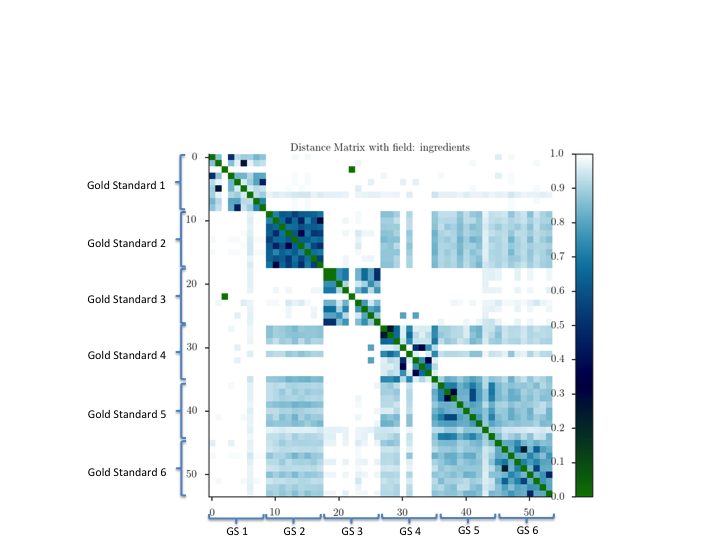
\includegraphics[width=15cm]{/Users/pierre/Documents/Telecom ParisTech/MS_Big_Data/ProjetDataMining/crawlers/Results Monop/CalculDistance/results_images/MatDist_nom_1/Diapositive1.png}
\end{figure}


    % Add a bibliography block to the postdoc
    
    
    
    \end{document}
